\begin{center}
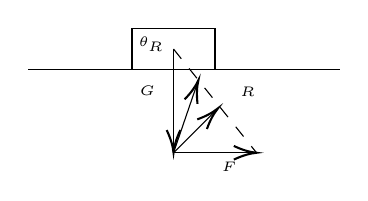
\begin{tikzpicture}[x=0.75pt,y=0.75pt,yscale=-1,xscale=1]
%uncomment if require: \path (0,300); %set diagram left start at 0, and has height of 300

%Straight Lines [id:da524357483065941] 
\draw    (140,130) -- (290,130) ;
%Shape: Rectangle [id:dp1562964743350983] 
\draw   (190,110) -- (230,110) -- (230,130) -- (190,130) -- cycle ;
%Straight Lines [id:da659959210580102] 
\draw    (210,120) -- (210,168) ;
\draw [shift={(210,170)}, rotate = 270] [color={rgb, 255:red, 0; green, 0; blue, 0 }  ][line width=0.75]    (10.93,-3.29) .. controls (6.95,-1.4) and (3.31,-0.3) .. (0,0) .. controls (3.31,0.3) and (6.95,1.4) .. (10.93,3.29)   ;
%Straight Lines [id:da223898729028551] 
\draw  [dash pattern={on 4.5pt off 4.5pt}]  (210,120) -- (250,170) ;
%Straight Lines [id:da7461771596827373] 
\draw    (210,170) -- (248,170) ;
\draw [shift={(250,170)}, rotate = 180] [color={rgb, 255:red, 0; green, 0; blue, 0 }  ][line width=0.75]    (10.93,-3.29) .. controls (6.95,-1.4) and (3.31,-0.3) .. (0,0) .. controls (3.31,0.3) and (6.95,1.4) .. (10.93,3.29)   ;
%Straight Lines [id:da7253181021320425] 
\draw    (210,170) -- (230.09,149.91) ;
\draw [shift={(231.5,148.5)}, rotate = 135] [color={rgb, 255:red, 0; green, 0; blue, 0 }  ][line width=0.75]    (10.93,-3.29) .. controls (6.95,-1.4) and (3.31,-0.3) .. (0,0) .. controls (3.31,0.3) and (6.95,1.4) .. (10.93,3.29)   ;
%Straight Lines [id:da030028220247521498] 
\draw    (210,170) -- (221.35,136.89) ;
\draw [shift={(222,135)}, rotate = 108.92] [color={rgb, 255:red, 0; green, 0; blue, 0 }  ][line width=0.75]    (10.93,-3.29) .. controls (6.95,-1.4) and (3.31,-0.3) .. (0,0) .. controls (3.31,0.3) and (6.95,1.4) .. (10.93,3.29)   ;

% Text Node
\draw (192,113) node [anchor=north west][inner sep=0.75pt]  [font=\tiny] [align=left] {$\displaystyle \theta _{R}$};
% Text Node
\draw (192.5,136.5) node [anchor=north west][inner sep=0.75pt]  [font=\tiny] [align=left] {$\displaystyle G$};
% Text Node
\draw (232,173) node [anchor=north west][inner sep=0.75pt]  [font=\tiny] [align=left] {$\displaystyle F$};
% Text Node
\draw (236.5,138) node [anchor=north west][inner sep=0.75pt]  [font=\tiny] [align=left] {$ $};
% Text Node
\draw (241,137) node [anchor=north west][inner sep=0.75pt]  [font=\tiny] [align=left] {$\displaystyle R$};


\end{tikzpicture}

\end{center}